

\newpage

\section{Multi-scalar modeling of residential dynamics}{Modélisation multi-scalaire des dynamiques résidentielles} % Chapter title

\label{app:sec:migrationdynamics} % For referencing the chapter elsewhere, use \autoref{ch:name} 

%----------------------------------------------------------------------------------------

% MigrationDynamics : exemple of multi-scale model structure

Nous avons effleuré dans le chapitre introductif les questions de mobilité (quotidienne et résidentielle) comme processus voisins de ceux qui nous ont occupé tout au long de ce travail, à une autre échelle et avec d'autres ontologies. Nous avons d'autre part suggéré l'ouverture vers des modèles multi-échelles comme un développement privilégié et une application relativement immédiate des briques préliminaires que nous avons forgé ici. Cet annexe présente brièvement un travail développant précisément ces deux points, dans le cas des dynamiques résidentielles des migrants ruraux dans le Delta de la rivière des Perles en Chine.


\stars


%----------------------------------------------------------------------------------------


\textit{Ce travail est le fruit d'une collaboration interdisciplinaire avec l'anthropologue \noun{Cinzia Losavio} (UMR CNRS 8504 Géographie-cités), dans le cadre du projet MEDIUM. Le texte produit en collaboration est ici adapté et traduit. Ces résultats ont été présenté à la conférence internationale Urban China 2017 comme \cite{losavio2017modeling}}.


\stars


%----------------------------------------------------------------------------------------


\bpar{
This paper introduces an agent-based model of regional migration dynamics, applied to the Mega-city Region of Pearl River Delta. It focuses on residential dynamics of migrants workers and aims at taking into account the variety of migrant's profiles, based on qualitative fieldwork observations. The extensive exploration of the model, both on synthetic and real-world configurations, yield several stylized facts of migration processes and specific effects of the regional geography, which can be used to inform migration policies. We postulate that such integrated modeling approaches will be more and more appropriate to study cities in China.
}{
Cette section introduit un modèle basé agent des dynamique de migration intra-régionales, appliqué à la Méga-city Region du Delta de la Rivière des Perles. Il se concentre sur les dynamiques résidentielles de travailleurs migrants et vise à prendre en compte la variété des profils des migrants, en se basant sur des observations qualitatives de terrain. L'exploration intensive du modèle, à la fois sur des configurations synthétiques et réelles, fournit des faits stylisés sur les processus de migration, et des effets spécifiques de la géographie régionale, qui pourraient être appliqués aux régulations des migrations. Nous supposons que de telles approches de modélisation intégrées seront par l'avenir de l'étude des villes chinoises.
}



\subsection{Introduction}{Introduction}

\paragraph{Context}{Contexte}


\bpar{
Over the last three decades, rural-to-urban migrant-workers have been a driving force for China's economy, raising attention on associated socio-economical issues. However, the importance of their economic diversity and social mobility has been poorly considered in the analysis of urban development strategy.
}{
Ces dernières décades, les travailleurs migrants du rural vers l'urbain ont été une force motrice pour l'économie chinoise, attirant l'attention sur les questions socio-économiques associées. Cependant, l'importance de leur diversité économique et la mobilité sociale ont été peu considérés dans l'analyse des stratégies de développement urbaines.
}

\bpar{
We use an agent-based model to simulate residential dynamics of migrants in Pearl River Delta (PRD) mega city region, taking into account the full range of migrants’ socio-economical status and their evolution. Mega-city regions have become a new scale of Chinese State regulation, and PRD represent the most prosperous and dynamic one in term of migration waves, standing as an ideal unit of analysis.
}{
Nous utilisons un modèle basé agent pour simuler les dynamiques résidentielles des migrants dans la méga-région urbaine du Delta de la Rivière des Perles (PRD), prenant en compte l'ensemble des statuts socio-économique des migrants et leur évolution. Les méga-régions urbaines sont devenues une nouvelles échelle de régulation pour l'Etat Chinois, et le PRD représente le plus prospère et dynamique en termes de vagues de migrations. Cela en fait ainsi une parfaite unité d'analyse.
}


\paragraph{Mega-city Regions}{Méga-régions urbaines}


\bpar{
Mega-city regions (MCRs) as defined by Florida, Gulden and Mellander are ``integrated sets of cities and their surrounding suburban hinterlands across which labour and capital can be reallocated at very low cost''~\cite{florida2008rise}. This urban configuration recalls what Gottmann defined as \emph{megalopolis}~\cite{gottman1961megalopolis} in reference to the north-east coast of the United States. Despite this affinity in their spatial and functional configuration, MCRs perform on a different scale than megalopolis: they operate at a regional as well as at a global scale. Indeed, one of the main characteristics of MCRs is their ``connectivity'': spatially, they branch out into nearby rural and metropolitan areas, and economically they grow beyond their physical border, becoming international. These densely populated regions do not have a single barycenter but merging into one another they turn into highly networked spaces connected through multiple nodes. The high density of connections and the polycentrism characterizing these new economic units facilitate migrations flows and encourage regional integration.
}{
Les \emph{Mega-city Regions} (MCR) sont définies par \cite{florida2008rise} comme ``\textit{des ensembles de villes intégrés et leur territoires suburbains environnants, au sein desquels le travail et le capital peuvent être réalloués à moindre coût}''. Cette configuration urbaine correspond à ce que \cite{gottman1961megalopolis} définit comme \emph{megapolis} en référence à la cote nord-est des Etats-unis. Malgré cette similarité dans leur configuration spatiale et fonctionnelle, les MCRs fonctionnent à une échelle différentes de celle de la megapolis : elles opèrent à la fois à une échelle régionale et à une échelle globale. En effet, l'une des caractéristiques principales des MCRs est leur connectivité : spatiallement elles s'étendent aux régions urbaines et métropolitaines proches, et économiquement elles ont un impact international, bien au delà de leur frontière physique. Ces régions densément peuplées n'ont pas un unique barycentre, mais consistent en de multiples centres fortement connectés. La forte densité de connections et le polycentrisme caractérisant ces nouvelles unités économiques facilitent les flux de migration et encouragent l'intégration régionale.
}


\bpar{
In China, the development of mega-city regions has started right after the implementation of the Open Door Policy in 1978. But it is the gradual decentralization of the State power - which occurred in the beginning of 1990 – that promote cities and more recently mega-city regions as a new scale of Chinese State regulation~\cite{IJUR:IJUR12437}. The process of rapid economic growth and urban development molds new densely populated and industrially dynamic mega-city regions, of which the Pearl River Delta (PRD)\footnote{The PRD Mega City Region consists of nine cities: the core cities are Guangzhou and Shenzhen, surrounded by Dongguan, Foshan, Zhongshan, Zhuhai, Huizhou, Jiangmen, and Zhaoqing. The model does not include Hong Kong and Macau, which are part of the PRD Mega Urban Region.} is the most obvious example. The area was designed in 1988 as a ``comprehensive economic reform area'', and was granted many ``one step ahead'' policies to attract foreign capital. Evolving into the most important exporter center since the economic reform, the Pearl River Delta represents the most dynamic MCR in terms of migration waves~\cite{IJUR:IJUR820}.
}{
En Chine, le développement des méga-régions urbaines a commencé juste après l'implémentation de la politiques des portes ouvertes en 1978. Mais c'est la décentralisation progressive du pouvoir de l'Etat, qui a eu lieu au début des années 1990, qui promeut les villes et plus récemment les méga-régions urbaines comme une nouvelle échelle de régulation de l'Etat Chinois~\cite{IJUR:IJUR12437}. Le processus de croissance économique rapide et le développement urbain conduisent à de nouvelles méga-régions urbaines densément peuplées et industriellement dynamiques, parmi lesquelles le Delta de la Rivière des Perles (PRD)\footnote{La \emph{Mega City Region} du PRD est composée de neuf villes : les villes coeur sont Guangzhou et Shenzhen, entourées de Dongguan, Foshan, Zhongshan, Zhuhai, Huizhou, Jiangmen, et Zhaoqing. Le modèle n'inclut pas Hong-Kong et Macao, qui font partie de la méga-région urbaine du PRD.} est l'exemple le plus représentatif. La zone a été choisie en 1988 comme une ``zone de réforme économique complète'', et il lui a été accordé de nombreuse politiques de ``pas en avant'' pour attirer le capital étranger. Evoluant vers le centre d'exportation le plus important depuis les réformes économiques, le Delta de la Rivière des Perles représente la MCR la plus dynamique en termes de vagues de migration~\cite{IJUR:IJUR820}.
}


\paragraph{Migrant Workers}{Travailleurs migrants}

\bpar{
Taking the PRD as the spatial unit of the model, we aim to reproduce migrant workers’ residential patterns taking into account the full range of their socio-economical status. Migration patterns and key related issues have extensively been studied from very diverse perspectives, ranging for example from racialization issues~\cite{dong2010policing} to big data analysis of their spatio-temporal behavior~\cite{2017arXiv170600682Y}. However, migrant workers are generally considered and treated as a uniform category, which stand at the bottom of the urban society, carrying the stigma of the rural household registration system. The rural-urban dual structure has been for years the only approach to define and understand migrant-workers, but the process of rapid economic growth China have been experiencing accelerated social transformation. We postulate that studying migrant workers, by merely considering their \emph{hukou} status and place of registration is not sufficient anymore to apprehend such a complex and diversified social category. Others aspects such as migrant workers economical, cultural and human capital should be taken into account.
}{
Considérant le PRD comme l'unité spatiale d'étude, nous visons à reproduire les motifs résidentiels des travailleurs migrants, en prenant en compte l'ensemble des possibilités de leur statut socio-économique. Les motifs de migration et les questions essentielles qui y sont rattachées ont été largement étudiés selon diverses perspectives, s'étendant par exemple de questions ethniques~\cite{dong2010policing} aux analyses par données massives de leur comportement spatio-temporel~\cite{2017arXiv170600682Y}. Cependant, les travailleurs migrants sont généralement considérés et traités comme une catégorie uniforme, qui est placée au bas de la société urbaine, portant les stigmates du système d'enregistrement rural. La structure duale rurale-urbain a depuis des années été l'unique approche pour définir et comprendre les travailleurs migrants, mais le processus de croissance économique rapide que la Chine a expérimenté a accéléré la transformation sociale. Nous postulons que l'étude des travailleurs migrants en considérant seulement leur statut de \emph{Hukou} et le lieu d'enregistrement n'est plus suffisant pour appréhender une telle catégorie sociale complexe et diversifiée. D'autres aspects comme le capital économique, culturel et humain des travailleurs migrants doit être pris en compte.
}


\bpar{
Especially three dimensions can help differentiate number of migrant-workers sub-categories: (i) the professional dimension, which not only determines migrants’ economical situation but also influences their trajectory and the duration of their staying in the city as well as their residential choice; (ii) the residential dimension which impacts all aspects of migrants’ urban lives – patterns of urban settlement, housing choices, residential conditions, relation with the city, neighborhood activities etc; (iii) the generational dimension.\footnote{The generational dimension is not taken into account in the model, as simulated dynamics correspond to rather short time scales, between 10 and 20 years.}
}{
En particulier, trois dimensions peuvent être utiles pour différencier un certain nombre de sous-catégories de travailleurs migrants : (i) la dimension professionnelle, qui détermine non-seulement la situation économique des migrants mais influence également leur trajectoires et la durée de leur séjour dans la ville ainsi que leurs choix résidentiels ; (ii) la dimension résidentielle qui influe sur l'ensemble des aspects des vies urbaines des migrants : établissements urbains, choix de logement, conditions résidentielles, relations à la ville, activités de voisinage, etc. ; (iii) la dimension de la génération\footnote{La dimension génération n'est pas prise en compte dans le modèle, puisque les dynamiques simulées correspondent à des échelles temporelles plutôt courtes, entre 10 et 20 ans.}.
}


\bpar{
All these sub-categories have different mobility patterns, that we simulate in the model. Considering this diversity and translating it in qualitative stylized facts that correspond to precise patterns of synthetic data, this model aims at establishing a new perspective for understanding China’s urban and regional mobility employing a more qualitative approach, specifying the mechanisms through which Party-State shape the parameters of migrants’ choices. 
}{
Toutes ce sous-catégories ont différents motifs de mobilité, que nous simulons dans le modèle. Considérant cette diversité et la traduisant en faits stylisés qualitatifs qui correspondent à des motifs précis de données synthétiques, ce modèle vise à établir une nouvelle perspective pour comprendre la mobilité résidentielle urbaine et régionale en Chine, en utilisant une approche plus qualitative par la spécification des mécanismes par lesquels l'Etat-Parti contrôle les paramètres des choix des migrants.
}




%%%%%%%%%%%%%%%%%%%%
\subsection{Model}{Modèle}


%%%%%%%%%%%%%%%%%%%%
\paragraph{Modeling Rural-urban migrations in China}{Modélisation des migrations rural-urbain en Chine}

% agent-based model in Urban Studies : http://journals.sagepub.com/doi/pdf/10.1177/0042098009346326
% http://en.cnki.com.cn/Article_en/CJFDTotal-CSFY200909013.htm
% http://www.tandfonline.com/doi/full/10.1111/j.1467-8306.2007.00559.x?scroll=top&needAccess=true : CA model of Desakota (rurban expansion)

%\paragraph{Modeling Rural-urban migrations}

%\cite{todaro1969model} classical equilibrium model

%\comment[JR]{\cite{2017arXiv170600682Y} : big data analysis of migrants spatio-temporal behavior}


\bpar{
Existing works in rural-urban migration modeling in China are mainly econometric studies, relying on census or on survey data. \cite{zhang2013measuring} estimate discrete choice models to study the trade-off between migration distance and earning difference. \cite{fan2005modeling} shows that gravity-based models can explain well inter-provincial migratory patterns, implying an underlying strong dominant aggregation processes. The positive association between wage gap and migration rates was obtained from time-series analysis in~\cite{zhang2003rural}. An empirical study of intra-urban migrants residential dynamics is done by~\cite{wu2006migrant}. \cite{xie2007simulating} uses an agent-based model to simulate the emergence of Urban Villages. To the best of our knowledge, there was no previous attempt in the literature to model regional migrations in China from an agent-based perspective.
}{
La plupart des travaux existant sur la modélisation de la migration rural-urbain en Chine sont principalement des études économétriques, qui se basent sur des données des sondages ou d'études ciblées. \cite{zhang2013measuring} estime des modèles de choix discrets pour étudier le trade-off entre distance de migration et différence de salaire. \cite{fan2005modeling} montre que des modèles gravitaires peuvent bien expliquer les motifs de migration inter-provinciaux, impliquant de forts processus dominants d'agrégation sous-jacents. L'association positive entre les écarts salariaux et les taux de migration a été obtenue à partir d'analyse de séries temporelles dans~\cite{zhang2003rural}. Une étude empirique des dynamiques résidentielles intra-urbaines des migrants est faite par~\cite{wu2006migrant}. \cite{xie2007simulating} utilise un modèle basé agent pour simuler l'émergence des villages urbains. Au meilleur de notre connaissance, il n'existe pas de tentative précédente dans la littérature pour modéliser les migrations régionales en Chine à partir d'une perspective basée agent.
}


%The case of Mexico was tackled by~\cite{de2007netlogo}, but in the particular case of a border-town, and underlying processes are furthermore fundamentally different.

 %\cite{silveira2006agent} : Ising model of rural-urban migration.
  %\cite{fernandez2005characterizing} : study of population characteristics to establish the relevance of a future ABM. \comment{I think later we should comment a bit more the litterature you cite here!}[yes of course]

%The idea of applying complexity paradigms to rural-urban migration is far from new, as~\cite{mabogunje1970systems} already theorized it in the frame of General System Theory, that for some is viewed as a precursor of complexity theories. \comment{Was there a particular study? If is we can be more precise at least on the country where this kind of pattern has been studied}[it is a fully theoretical paper (although the empirical inspirations seem to be from Nigeria). the citation was more to justify our theoretical and methodological background, we'll have to think if it is really appropriate]

%Following a logic of \emph{Pattern-oriented modeling}~\cite{grimm2005pattern}, combined with recent advances in multi-modeling~\cite{cottineau2016back}, one can use agent-based models as powerful tools to test qualitative hypothesis, with a reasonable need for empirical data through toy-models or hybrid models.



\paragraph{Model}{Modèle}


\bpar{
The model is designed to include targeted stylized facts and experiments, in particular the role of the socio-economic structure of migrant population. More precisely, a recent shift in socio-economic structure of migrating population was observed, including a rise of middle-income migrants and a relativisation of the role of \emph{Hukou} in migration dynamics. The core of the model is thus centered on the exploration of the impact of a varying population economic structure for migrants on system dynamics, and the influence of government migration policies.
}{
Le modèle est conçu pour inclure des faits stylisés précis et des expériences associées, en particulier le rôle de la structure socio-économique de la population de migrants. Plus précisément, un changement récent dans la structure socio-économique de la population migrante a été observée, incluant une augmentation du nombre de migrants aux salaires médians et une relativisation du rôle du \emph{Hukou} dans les dynamiques migratoires. Le coeur du modèle est pour cette raison centré sur l'exploration de l'impact d'une variation de la structure économique de la population des migrants sur les dynamiques du système, et l'influence des politiques migratoires gouvernementales.
}

\bpar{
 The region is represented in the model by $N$ patches, characterized by their population $P_i(t)$ and an economic structure $E_i^{(c)}(t)$ giving a potential number of jobs for socio-economic classes $c$. The associated effective number of workers is denoted by $W_i^{(c)}(t)$. For the sake of simplicity, we assume a discrete number of classes. At initial time, the variables are initialized either following a synthetic data generation process (see below), or from real geographical data (abstracted and simplified to fit our context). 
}{
La région est représentée dans le modèle par $N$ patches, caractérisé par leur population $P_i(t)$ et une structure économique $E_i^{(c)}(t)$ qui représente un nombre potentiel d'emplois pour une classe socio-économique $c$. Le nombre effectif de travailleurs associés est noté $W_i^{(c)}(t)$. Dans un souci de simplicité, nous supposons un ensemble discret de classes. A l'instant initial, les variables sont initialisées soit selon un processus de génération de données synthétiques (voir ci-dessous), ou à partir de données géographiques réelles (abstraites et simplifiées pour répondre à notre contexte).
}

\bpar{ 
Urban Centers are characterized by aggregated population $\tilde{P}_k(t)$ and corresponding economic variables $\tilde{E}_k^{c}(t)$. An agent is a household of migrants, with location for residence and job. Socio-economic structure of the population is captured by the distribution of wealth $g(w)$, which are then stratified into categories. At a given time, the utility difference between not moving and moving to cell $j$ from cell $i$, for a category $c$ is given by
}{
Les centres urbains sont caractérisés par une population agrégée $\tilde{P}_k(t)$ et les variables économiques correspondantes $\tilde{E}_k^{c}(t)$. Un agent est un foyer de migrants, avec une localisation résidentielle et pour le travail. La structure socio-économique de la population est capturée par la distribution de richesse $g(w)$, qui est ensuite stratifiée en catégories. A un instant donné, la différence d'utilité entre l'action de relocalisation de la cellule $j$ vers la cellule $i$ et rester sur place, pour une catégorie $c$, est donnée par
}


\[
\Delta U_{i,j}^{(c)}(t) = \frac{Z_j^{(c)}- Z_i^{(c)}}{Z_0} + \gamma \cdot \frac{C_i^{(c)}- C_j^{(c)}}{C_0} - u_i^{(c)} - h_j^{(c)}
\]

\bpar{
where $Z_i^{(c)}$ is generalized accessibility given by 
}{
avec $Z_i^{(c)}$ une mesure d'accessibilité généralisée définie comme
}

\[
Z_i^{(c)} = P_i \cdot \sum_k \left[E_k^{(c)}-W_k^{(c)}\right]\cdot \exp{\left(\frac{-d_{ij}}{d_0}\right)}
\]

\bpar{
with $d_{ij}$ effective travel distance\footnote{as the model does not focus on the role of transportation, we take euclidian distance, and $d_0$ captures typical commuting distance in both public transportation or car. A more complicated model could include an explicit transportation network and modal choice depending on socio-economic category.} and $d_0$ commuting characteristic distance ; the parameter $\gamma$ is the ratio giving the relative importance of life cost compared to accessibility in the migration decisions ; $C_i^{(c)}$ is the cost of life which is a function of cell and city variables, that will be taken as $C_i^{(c)} \propto P_i^{\alpha_0}\cdot  \tilde{P}_i^{\alpha_1}$ ; $u_i^{(c)}$ a baseline aversion to move and $h_j^{(c)}$ an exogenous variable corresponding to regulation policies; $Z_0$ and $C_0$ dimensioning parameters.
}{
avec $d_{ij}$ une distance effective de trajet\footnote{Comme le modèle ne se concentre pas sur le rôle des transports, nous prenons la distance euclidienne, et $d_0$ capture une distance typique de migration pendulaire à la fois par transport public et voiture. Un modèle plus compliqué pourrait inclure un réseau de transport explicite ainsi que des choix modaux dépendants des catégories socio-économiques.} et $d_0$ distance de migration pendulaire typique ; le paramètre $\gamma$ est un rapport donnant l'importance relative du coût de la vie en comparaison à l'accessibilité dans les décisions migratoires ; $C_i^{(c)}$ est le coût de la vie qui est une fonction à la fois de la cellule et des variables de la ville, que nous prenons comme $C_i^{(c)} \propto P_i^{\alpha_0}\cdot  \tilde{P}_i^{\alpha_1}$ ; $u_i^{(c)}$ est une aversion au mouvement de référence et $h_j^{(c)}$ une variable exogène correspondant aux politiques de régulation ; $Z_0$ et $C_0$ sont des paramètres de dimensionnement.
}
 
% \comment[JR]{comparer a des modeles standard d'eco urbaine pas si different avec utilite cout transport access etc ; comparer utilite de Barthelemy}

 
\bpar{
At each time step, the system evolves sequentially according to the following rules : 
\begin{enumerate}
	\item cities-level variables are updated and distributed across patches variables (in our first experiments, we will assume short time scale and skip this step)
	\item new migrants enter the region and lean on social network to settle
	\item migration occur within the region, randomly drawn from discrete choice probabilities obtained with the above utility difference between two patches
	\item Migrants update their wealth and eventually economic category, according to an abstract ``quality of place'' that we associate to per-capita GDP which follows a scaling law of population.
\end{enumerate}
}{
A chaque pas de temps, le système évolue séquentiellement selon les règles suivantes :
\begin{enumerate}
	\item les variables au niveau de la ville sont mises à jour et distribuées aux variables de patch (dans les premières expériences, nous supposerons une courte échelle temporelle et sauterons cette étape) ;
	\item de nouveaux migrants entrent dans la région et se fient à leur réseau social pour s'établir ;
	\item les migrations ont lieu dans la région, tirées aléatoirement à partir des probabilités de choix discrets obtenues avec les différences d'utilités entre patches données ci-dessus ;
	\item les migrants mettent à jour leur richesse et possiblement leur catégorie économique, selon une ``qualité du lieu'' abstraite que nous associons au GPD par tête qui suit une loi d'échelle de la population.
\end{enumerate}
}



%%%%%%%%%%%%%%%%%
\subsection{Results}{Résultats}


\bpar{
The model is implemented in NetLogo, the open source implementation being available with results at \url{https://www.github.com/JusteRaimbault/MigrationDynamics}. We explore the model on synthetic city systems first, to isolate results due to processes from results due to geographical configuration. With such a random model where many parameters cannot be given directly a real-world value, it is necessary to explore intensively the parameter space to obtain robust conclusions. Using the software OpenMole~\cite{reuillon2013openmole}, we proceed to 1,599,495 simulations of the model on computation grid, achieving 15 years of equivalent CPU in around 2 days. We validate the model internally by checking the statistical convergence of indicators.
}{
Le modèle est implémenté en NetLogo, l'implémentation ouverte étant disponible avec les résultats à \url{https://www.github.com/JusteRaimbault/MigrationDynamics}. Le modèle est d'abord exploré sur des systèmes de villes synthétiques, afin d'isoler les résultats dus aux processus en eux-même des résultats dus à la configuration géographique. Avec un tel modèle stochastique pour lequel de nombreux paramètres ne peuvent être fixé par des valeurs observées, il est nécessaire d'explorer de manière extensive l'espace des paramètres pour obtenir des conclusions robustes. Grâce au logiciel OpenMole~\cite{reuillon2013openmole}, nous procédons à 1,599,495 simulations du modèle sur grille de calcul, réalisant autour de 15 ans de calcul en équivalent CPU en environ 2 jours. Nous validons le modèle de manière interne en vérifiant la convergence statistique des indicateurs.
}


\bpar{
From the baseline experiments we learn that : (i) when migrants have a high propensity to move, the spatial repartition of jobs becomes suboptimal in intermediate regimes of stochasticity, corresponding to a regime where congestion dominates; % More precisely, we use a ``Random Utility'' specification for migrants' decisions, that includes a parameter $\beta$ that represents a ``level of randomness'' (or stochasticity) : when it goes to 0, migrations are totally random and without any sense, when it goes to infinity, migrants follow deterministically the best choice between staying and going to the best migration patch (depending on the sign of $\Delta U$). For intermediate values of $\beta$, we observe this congestion phenomenon.
 (ii) the congestion regime corresponds to a linear decrease of job distance with randomness, meaning that social determinism creates spatial inequalities; % It means that proximity to job is correlated with more congestion, but there is no direct causality between the two, both are outcome of model processes;
 (iii) changing the relative importance of accessibility does not affect much the aggregated dynamics: an increased gain in mobility produced by policies such as individual transportation subsidies will have no effect on migrations patterns. %Accessibility is a generic notion to capture patterns of accessibility to urban functions and amenities ; in our case we use generalized Hansen accessibility, which can be understood in a simplified way number of jobs available to the population within a spatial range.
(iv) configurations with an intermediate value of move aversion (in which real configurations fall) yield a negative feedback effect of time, witnessing a progressive saturation. In a ``U-shape'' manner, very mobile or very fixed configurations yield positive feedback of time. We then turn to specific experiments.
}{
Les expériences de contrôle (valeur de référence des paramètres) fournissent les faits stylisés suivants sur les dynamiques intrinsèques au coeur du modèle :
\begin{enumerate}
	\item Lorsque les migrants ont une forte potentialité de mobilité, la répartition spatiale des emplois devient sous-optimale dans des régimes intermédiaires de stochasticité (au sens des valeur prises par le paramètre de choix discrets), ce qui correspond à un régime où la congestion domine.
	\item Ce régime de congestion implique une décroissance linéaire de la distance à l'emploi avec la diminution du caractère aléatoire, ce qui signifie que le déterminisme social crée des inégalités spatiales.
	\item L'importance relative de l'accessibilité influe très peu les dynamiques agrégées. Ainsi, un gain croissant en mobilité (c'est à dire une importance accrue pour l'accessibilité), qui peut être encouragé par des politiques locales telles des subventions, n'aura que très peu d'effet sur les motifs de migration.
	\item Les configurations avec des valeurs intermédiaires de l'aversion au mouvement (dans lesquelles la situation réelle se trouve) induisent un effet de feedback négatif du temps au cours des trajectoires, témoignant d'une saturation progressive. Dans un comportement ``en-U'', les configurations très mobiles et celles très stables donnent un effet positif du temps (augmentation du nombre de migrations).
\end{enumerate}
Nous étudions ensuite des expériences ciblées.
}



\bpar{
Adding categorization does not change the qualitative behavior of the model. % It does not mean that categorization (based on professional qualifications, education, and economic situation) does not influence the migration behavior. In practice for example the points-based hukou system favoring “talents” – people with more qualifications, with stable job and economic situation etc. – can have a significant influence on migration behavior. It changes the migration behavior for individuals, but not the global qualitative picture of the previous stylized facts. %I have to think more on this and I totally agree on your second point : an interesting thing to try when testing the Hukou policies in the model is to check if we have the same phenomenon, and then to compare the effectiveness of policies at the individual level (impact on migrants trajectories) to the global level (behavior of the model).
The lower category appears more vulnerable to spatial inequalities created by social determinism. Concerning the influence of economic parameters, namely income inequality and income growth, we find that : (i) larger income inequalities yield stronger spatial inequities in job accessibility; (ii) larger enrichments when migrating induces a suboptimal regime for the upper category.
}{
L'ajout des catégories socio-économiques ne change pas fondamentalement le comportement qualitatif du modèle. La catégorie la plus basse semble cependant plus vulnérable aux inégalités spatiales induites par le déterminisme spatial. Concernant l'influence des paramètres économiques, en particulier les inégalités de revenu et la croissance des revenus, nous trouvons que : (i) de plus fortes inégalités de revenus induisent de plus fortes inégalités spatiales dans l'accessibilité à l'emploi ; (ii) une croissance des revenus plus forte (un enrichissement plus grand) lors d'une migration conduit à un régime sous-optimal pour la catégorie supérieure.
}


\bpar{
The application of the model on the real population and economic configuration of Pearl River Delta slightly changes conclusions: we witness for example the emergence of optimal behavior ranges for the commuting distance indicators. It means that incentives for migrations have to be specifically tuned depending on the region configuration. Other conclusions mainly hold and are therefore process-specific.
}{
L'application du modèle sur la configuration observée pour la population et les emplois dans le delta de la rivière des Perles change légèrement les conclusions : celle-ci témoigne par exemple de plages optimales pour les paramètres comportementaux au regard des indicateurs de distance de mobilité pendulaire. Cela signifie que les incitations aux migrations doivent être spécifiquement conçues selon la configuration de la région. La plupart des conclusions tirées précédemment tiennent toujours, et sont ainsi spécifiques au processus considérés.
}




\paragraph{Discussion}{Discussion}


\bpar{
A last application we are currently developing is testing the impact of localized regulation policies, i.e. having the term $h_j^{(c)}$ varying across cities and across categories, what corresponds to policies effectively observed in practice. This various stylized facts listed above may furthermore inform more general policies, such as the impact of mobility or the existence of optimal regimes for intermediate values of randomness. Further work may consist in a calibration of the model on migration trajectories with appropriate datasets, but also in a feedback of simulation results on qualitative fieldwork, trying to compare to concrete real situations.
}{
Une dernière application en cours de développement est l'exploration de l'impact de politiques de régulation localisées, i.e. en ayant le terme $h_j^{(c)}$ qui varie selon les villes et selon les catégories socio-économiques, ce qui correspondrait à des politiques effectivement observées en pratique. Les divers faits stylisés décrits précédemment peuvent de plus être porteurs de sens pour l'élaboration de politiques plus générales, comme l'impact d'une mobilité accrue, ou bien l'existence de régimes optimaux pour des valeurs intermédiaires du caractère aléatoire. Un développement futur pourra consister en une calibration du modèle sur des trajectoires de migration avec les jeux de données appropriés, mais également en un retour des résultats de simulation sur le travail de terrain qualitatif, en les comparant aux situation concrètement observées.
}

% reflexion sur controle d'un complex system : attention requisite complexity - modele fit et action dans certain regime seulement, mais variables ``cachees'', comme non lineaire peut bifurquer sans qu'on comprenne pourquoi.


\bpar{
Our modeling entreprise is aimed at being integrated, as the model is initially built with taking in consideration qualitative observations from fieldwork, and as its outputs shall in return inform qualitative research. We believe that such integrated modeling approaches will be important tools in the future of Urban China research, in particular because of the emergence of new urban regimes in Chinese cities that were never observed somewhere else before, making difficult the use of some of previous empirical knowledge on cities.
}{
Cette entreprise de modélisation vise à être intégrée, puisque le modèle est initialement construit en prenant en considération des observation qualitative du travail de terrain\footnote{Pour rappeler le contexte dans le cadre plus général de la thèse, il ne s'agit pas du travail de terrain décrit en~\ref{sec:qualitative}, mais de celui de \noun{Cinzia Losavio} réalisé dans le cadre de sa thèse en cours (voir contributions ci-dessus).}, et ses sorties devraient en retour être utiles pour la recherche qualitative. Nous sommes convaincus que de telles approches de modélisation intégrée seront des outils importants pour le futur de la recherche Urbaine en Chine, en particulier en lien avec l'émergence de nouveaux régimes urbain dans les villes chinoises qui n'ont jamais été observés ailleurs auparavant, rendant difficile l'utilisation de certaines des connaissances empiriques précédentes sur les villes.
}




%%%%%%%%%%%%%%%
\begin{figure}%[h!]
\includegraphics[width=0.72\linewidth]{Figures/MigrationDynamics/model}
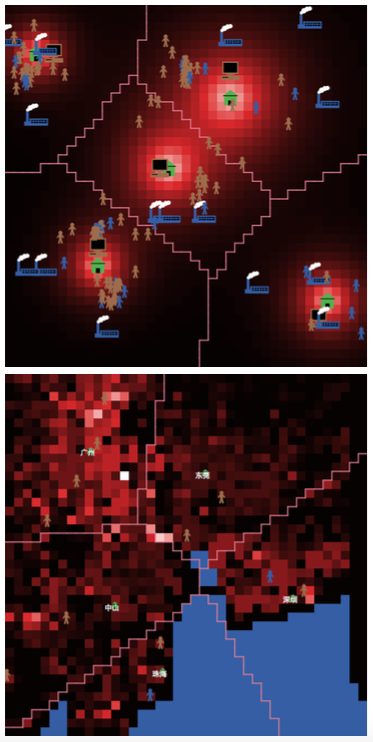
\includegraphics[width=0.22\linewidth]{Figures/MigrationDynamics/examples}
\appcaption{(Left) Multi-scale schema of processes included in the model. (Right) Examples of regional population configuration, for a synthetic city system (top) and Pearl River Delta (bottom).\label{app:fig:migrationdynamics:model}}{\textbf{Structure du modèle de migrations intra-régionales.} (\textit{Gauche}) Schéma des processus pris en compte et des agents, dans une perspective multi-scalaire\label{app:fig:migrationdynamics:model}}
\end{figure}
%%%%%%%%%%%%%%%



%%%%%%%%%%%%%%%
\begin{figure}[h!]
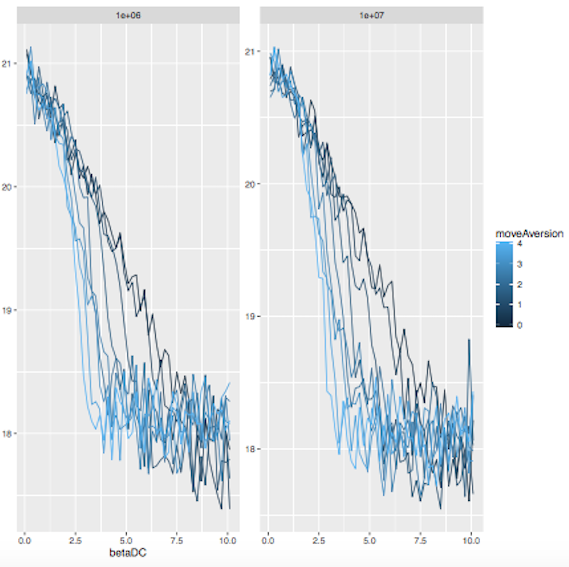
\includegraphics[width=0.49\linewidth]{Figures/MigrationDynamics/baseline_jobdist0.png}
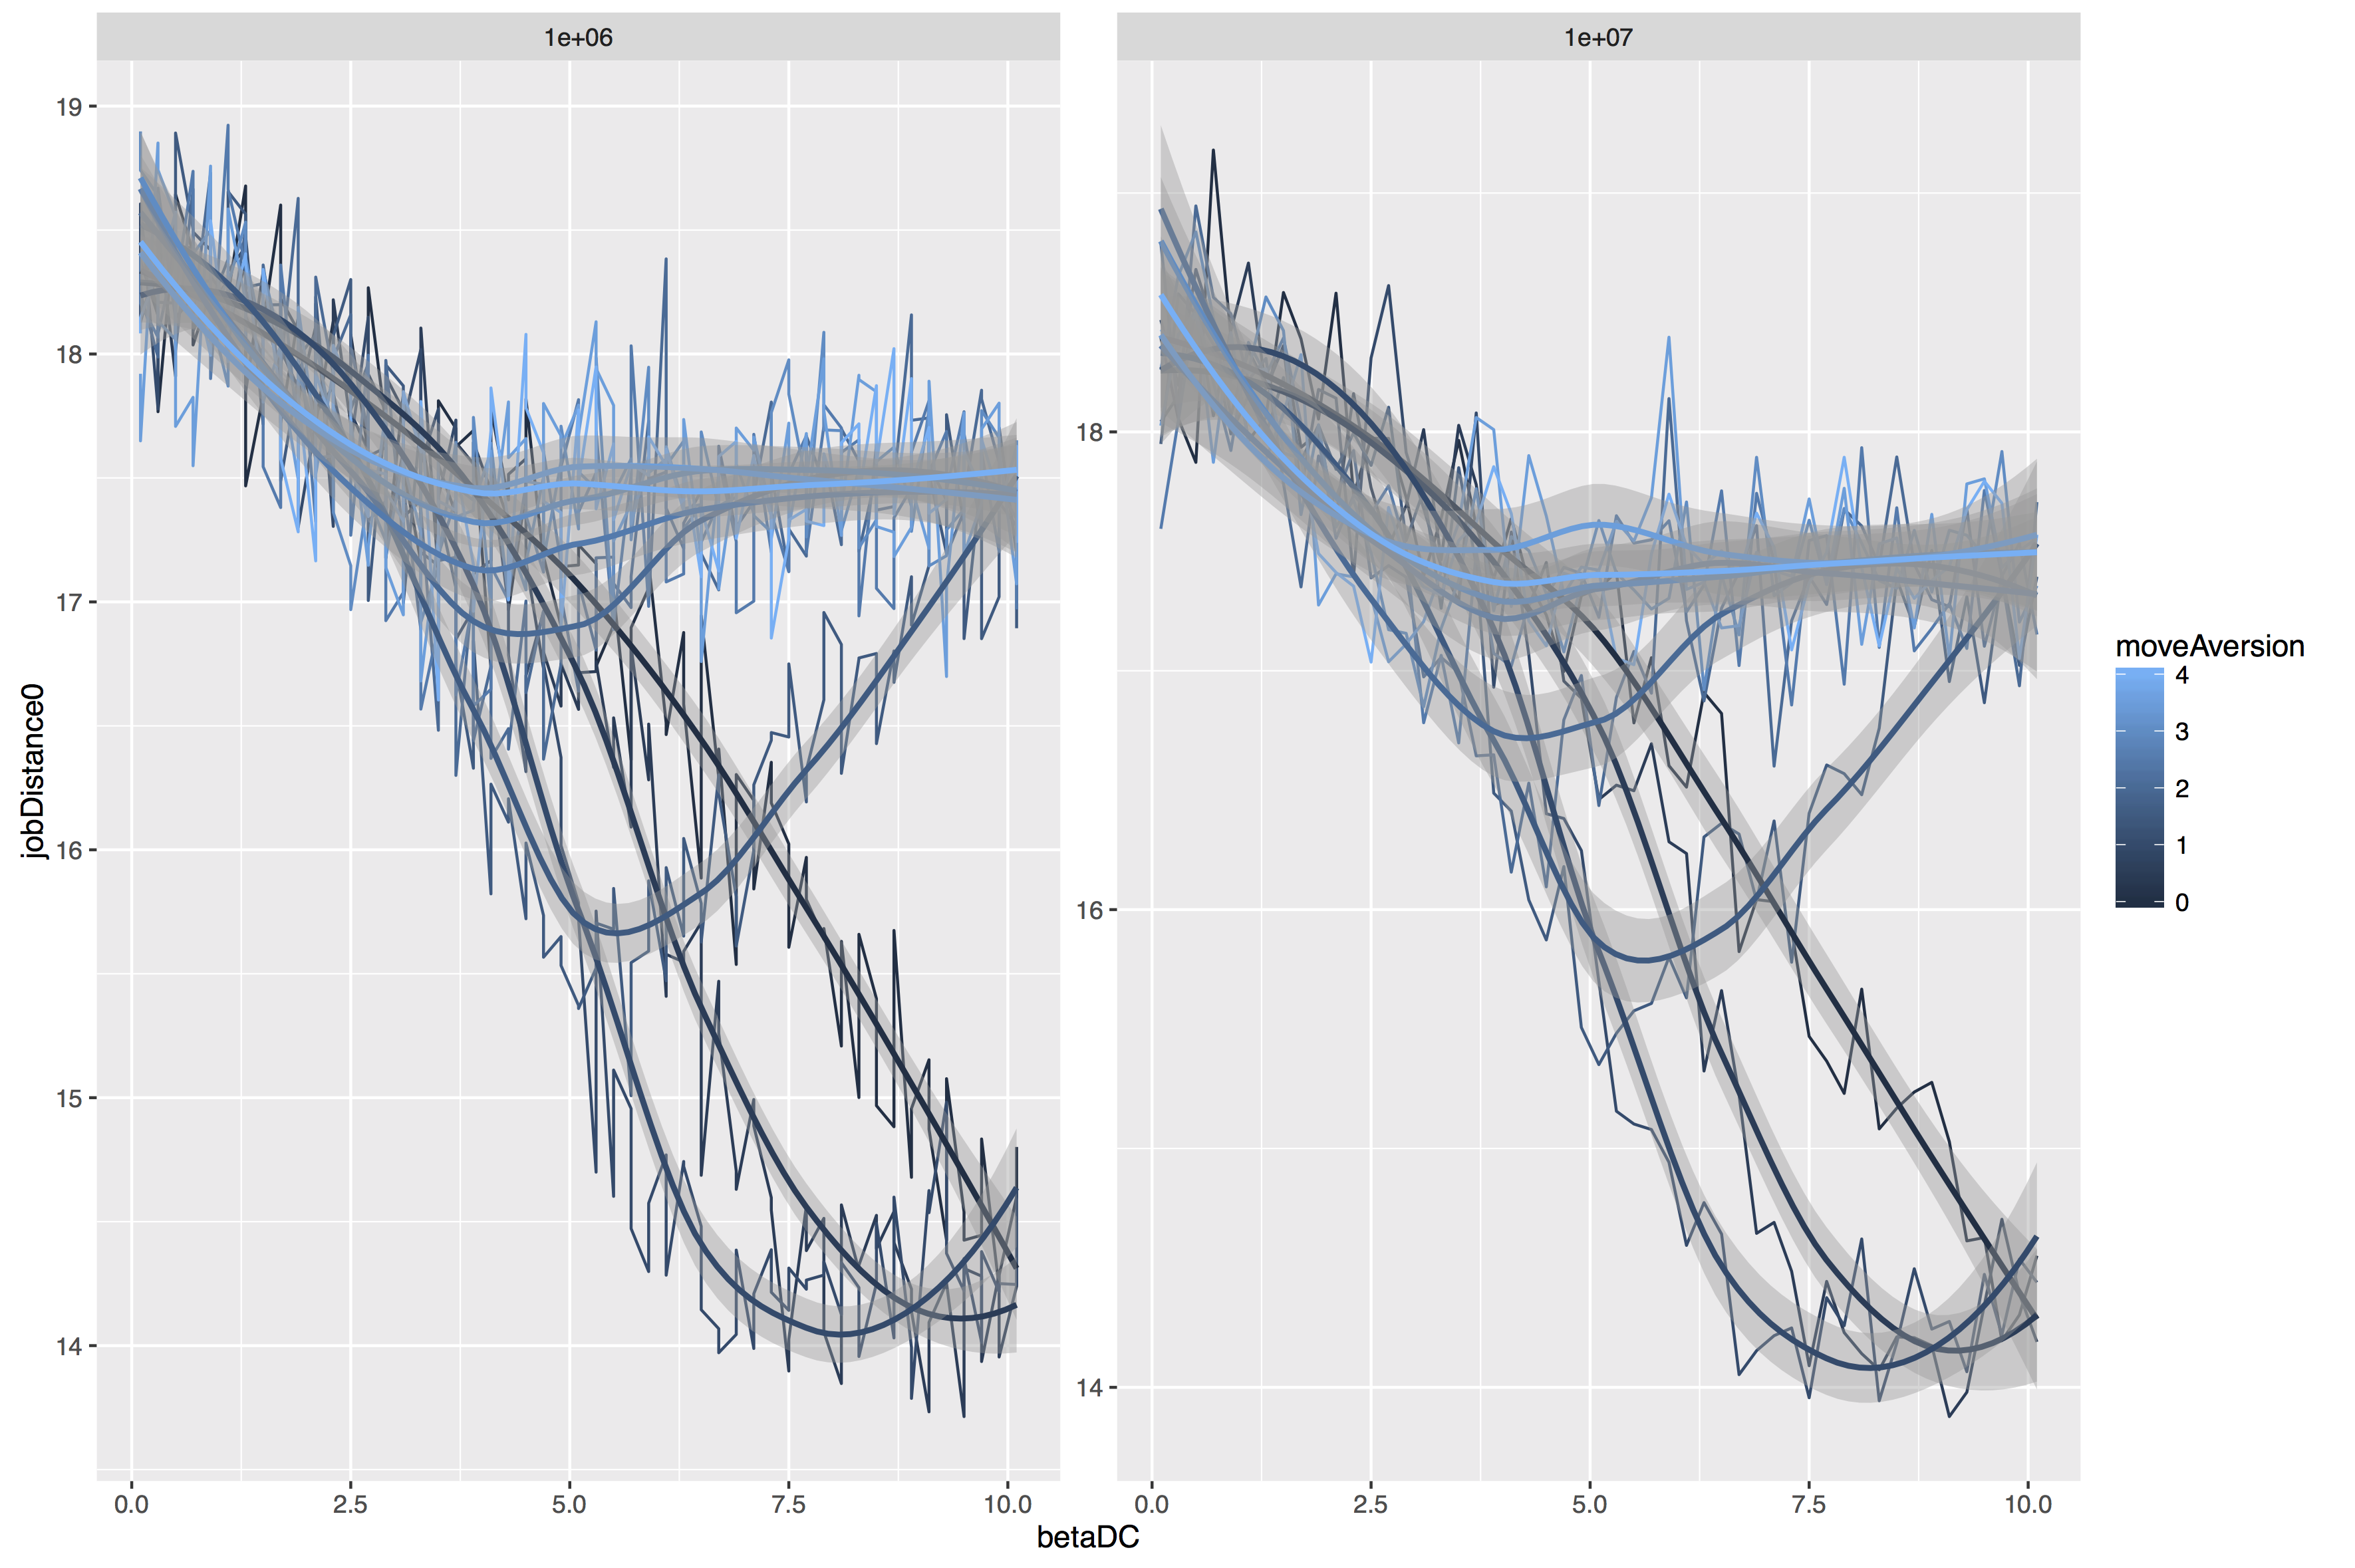
\includegraphics[width=0.49\linewidth]{Figures/MigrationDynamics/real_indicjobDistance0_smoothed.png}
\appcaption{}{Comparison of average distance to jobs for the lowest economic category, as a function of the randomness parameter $\beta$, between synthetic city systems (two left plots) and real configuration (two right plots). The color gives the constant move aversion $u_i^{(c)}$ and plots are given for two values of cost-accessibility ratio $\gamma$. We witness the apparition of optimal values of $\beta$ in the real situation, probably caused by the geography.\label{fig:model}}
\end{figure}
%%%%%%%%%%%%%%%


\newpage




%\begin{enumerate}
%\item Cities mesoscopic variables $\tilde{P}_k(t)$ and $\tilde{E}_k^{c}(t)$ are deterministically updated. Population follows the very simple assumption of the expectancy of a Gibrat's law, i.e. $\tilde{P}_k(t)= g_k \cdot \tilde{P}_k(t-1)$. Economy follows a scaling law of population: $\tilde{E}_k^{(c)}(t) = E_k^{(c,0)}\cdot \left(\frac{\tilde{P}_k(t)}{P_0}\right)^{\gamma_k^{(c)}}$.

%\item Patches variables are updated conditionally to the new aggregated values. For population, we adapt the aggregation-diffusion process detailed in~\cite{raimbault2016calibration}: a density ceil is introduced and diffusion is replaced by spatial noise. More precisely, let $\Delta \tilde{P}_k(t) = \tilde{P}_k(t) - \tilde{P}_k(t-1)$. \comment{less clear for me}[this part is unfinished indeed]

%\item A number $M$ of new migrants, enters the region. They lean on social network %(关系,guanxi) \comment{(CL) ADD EXPLICATIVE NOTE}
%to first settle in the city and agglomerate following a preferential attachment by place of origin.
%\item Migration occur following a discrete choice dynamics : the probability to move to cell $j$ is given by

%\[
%\Pb{i\rightarrow j | c} = \frac{\exp{\left(\beta\cdot U_j^{(c)}\right)}}{\sum_k \exp{\left(\beta\cdot U_k^{(c)}\right)}+\exp{\left(U_{stay,i}^{(c)}\right)}}
%\]

%what simplifies into a reduced form, with $\beta' = \frac{\beta}{Z_0}$, $\gamma' = \frac{\gamma}{Z_0C_0}$ and $\tilde{u},\tilde{h}$ accordingly rescaled variables, using the above utility expression :

%\[
%\Pb{i\rightarrow j | c} = \frac{\exp{\left(\beta'\cdot \left[\Delta Z_{i,j}^{(c)} - \gamma' \cdot \Delta C_{i,j}^{(c)} - \tilde{u}_i^{(c)} - \tilde{h}_j^{(c)} \right] \right)}}{1 + \sum_k {\exp{\left(\beta'\cdot \left[\Delta Z_{i,k}^{(c)} - \gamma' \cdot \Delta C_{i,k}^{(c)} - \tilde{u}_i^{(c)} - \tilde{h}_k^{(c)} \right] \right)}}}
%\]

%Residential movement is drawn randomly according to these probabilities, and jobs are chosen around new residence following an exponentially decreasing probability.

%\item Migrants update their wealth and eventually economic category, according to an abstract ``quality of place'' that we associate to per-capita GDP which follows a scaling law of population

%population / max-population * [city-population] of owning-city / economic-p0
% note : tunable function : test its role !

%\[
%w = w\cdot \left( 1 + g_{w} \frac{P_i}{\max P_j} \cdot \frac{\tilde{P}_k}{\max \tilde{P}_l} \right)
%\]

%\end{enumerate}


%\paragraph{Indicators}

%The outcome of the model has many dimensions, and is measured through the following indicators :

%\begin{itemize}
%\item Total migrants wealth gain
%\item Total migrants social mobility
%\item Cumulated utility difference in migrations: when someone migrates, it corresponds to a given utility gain $\Delta U$ : this indicator is $\sum \Delta U^{(c)}$ on all realized migrations for each category.
%\item Inequalities are captured by the final ratio between socio-economic categories
%\end{itemize}


%\paragraph{Synthetic Data Generation}

%A synthetic mega-city region is generated following simple stylized facts for systems of cities. A polycentric structure, each center having an exponential density decay, is created with random coordinates for centers. Population of centers follow a rank-size law of slope 1.2.


%\paragraph{Parameters}

%We summarise main parameters in table~\ref{tab:parameters}.

%\begin{table}
%\caption{Summary of main parameters\label{tab:parameters}}
%\bigskip
%\centering
%\begin{tabular}{ |c|c|c|c| } 
%\hline
%Parameter & Name & Values & Process  \\\hline
%$\gamma$ & Cost/Accessibility ratio & $\log\gamma \in \left[5;8\right]$ & Mobility \\ 
%$u_0$ & Move aversion & $u_0\in\left[0;5\right]$ & Risk aversion \\ 
%$\beta$ & Discrete Choices & $\beta\in \left]0;+\infty\right[$ & Determinism \\ 
%$g_w$ & Income Growth & $g_w \in \left[0;1\right]$ & Wealth Increase  \\
%$d_0$ & Accessibility Decay & $d_0\in \left]0;+\infty\right[$ & Accessibility \\ 
%$\sigma$ & Wealth dispersion & $\sigma\in \left[0.1;1.0\right]$ & Economic Inequalities \\ 
%\hline
%\end{tabular}
%\end{table}






%\todo{
%Next steps :
%\begin{itemize}
%\item Full exploration on synthetic data : model behavior
%\item Stylization and scenarization of real PRD configuration, model behavior on real and hybrid configurations
%\item Targeted experience plans (e.g. : role of economic diversity, influence of state regulation)
%\item Iterative further construction/multi-modeling (e.g. generations)
%\end{itemize}
%Expected Results :
%\begin{itemize}
%\item Impact of processes linked to migrants diversities on emergent dynamics
%\item Explore or unveil state strategies (through regulations or companies control \comment{why companies control ?}[I had in mind a possible action on company locations ?])
%\end{itemize}
%}



%%%%%%%%%%%%%%%%%%%%
%\subsection{Model Validation and Baseline Exploration}

%\paragraph{Internal validation} 

%statistical consistence : cf Fig.~\ref{fig:statistical-valid} ; system trajectories ; path-dependency.

%%%%%%%%%%%%%%%%
%\begin{figure}
%\centering
%\includegraphics[width=0.48\textwidth]{figures/baseline_hist_indivMigrations_colorbetaDC}
%\includegraphics[width=0.48\textwidth]{figures/baseline_hist_jobDistance0_colorbetaDC}
%\caption{Statistical distributions of number of individual migrations and wealth gain over 50 runs, for some example parameter points}
%\label{fig:statistical-valid}
%\end{figure}
%%%%%%%%%%%%%%%%




%\paragraph{External validation : baseline behavior}

%We first establish the behavior of the model on the simplest baseline situation, to which will be compared more complex parameter configurations. The baseline assumes no city growth ($g_k=1$), no external migration ($M=0$), no income growth ($g_{w}$), $u_i$ is fixed at a constant value $U_0$ and we have only one economic category. Fig.~\ref{fig:baseline-indics} show indicator values across the parameter space.

%We extract the following stylized facts from model behavior :
%\begin{itemize}
%\item As expected, we observe a phase transition in number of migrations for increasing $\beta$ ; the transition points increases when $u_0$ decreases, until the model follows a change in qualitative behavior (bifurcation ?) : increasing $\beta$ first produces a peak in migrations before they fall down again. The increase above 1 migration per migrant and per time step is possible by the disappearance of some of them due to a saturation of jobs. \textit{When migrants have a high propensity to move, the spatial repartition of jobs becomes suboptimal in intermediate regimes of stochasticity, corresponding to a regime where congestion dominates.} \comment{fact to be compared with the real config, maybe it is due to the spatial structure ; try to trickle also job number parameters, meta-parameter of synthetic system shape.}
%\item The previous observation is consistent with the behavior of the average distance to job (this plot is quite noisy as it depends on spatial configuration, stabilizing it would thus need supplementary repetitions, as the exploration for sensitivity of meta-parameters) : it always decreases with $\beta$, but individual move repulsion changes the shape. Low values give a linear decrease of job distance with $\beta$, whereas high values produce a saturating curve that becomes constant. \textit{The congestion regime corresponds to a linear decrease of job distance with randomness, meaning that social determinism creates spatial inequalities.}
%\item Not sensitive to $\gamma$ : the sensitivity to ratio cost/accessibility is very low \comment{(CL) to job or to city ?}[(JR) jobs, we work with generalized accessibility, see below], what may be due to the dependence of dynamics to outliers of utility distributions : its central shape changes a lot with it but not extreme values. \textit{Changing the relative importance of accessibility does not affect much the aggregated dynamics : an increased gain in mobility produced by policies for examples will have no effect on migrations patterns.} \todo{plot the patch distrib of utilities ? (in netlogo) $\rightarrow$ some examples }
%\item Temporal Dynamics : Fig.~\ref{fig:migr-diff}. The dependence of dynamics to parameter is much richer ; we observe a transition from a maximum, to a min, and then a max again. In configurations averse to move, time has a positive feedback on migrations ; intermediate situations show a negative feedback (progressive saturation in time) ; to switch again to a positive feedback in most mobile situations. \textit{Configurations with an intermediate value of move aversion (in which real configurations fall) yield a negative feedback effect to time, witnessing a progressive saturation. In a ``U-shape'' manner, very mobile or very fixed configurations yield positive feedback of time.} \comment{(JR) note : this directs to the exploration of not constant but proba distrib for $u_i$ ; or function of something ? no it is an externality !}
%\end{itemize}



%%%%%%%%%%%%%%%%%
%\begin{figure}
%\centering
%\includegraphics[width=0.48\textwidth]{figures/baseline_indicdeltaU0}
%\includegraphics[width=0.48\textwidth]{figures/baseline_indicindivMigrations}\\
%\includegraphics[width=0.48\textwidth]{figures/baseline_indicjobDistance0}
%\includegraphics[width=0.48\textwidth]{figures/baseline_indicutilitiesDecOrigin0_5}
%\caption{Model behavior, averaged over 50 runs, for a baseline configuration.}
%\label{fig:baseline-indics}
%\end{figure}
%%%%%%%%%%%%%%%%%


%%%%%%%%%%%%%%%%
%\begin{figure}
%\centering
%\includegraphics[width=\textwidth,height=0.3\textheight]{figures/migr-diff-final}
%\caption{Difference in number of migrations between initial and final state of the model (relatively robust to final time).}
%\label{fig:migr-diff}
%\end{figure}
%%%%%%%%%%%%%%%%%



%%%%%%%%%%%%%%%%%%%%
%\subsection{Stylized Facts}

%\paragraph{Role of economic categories}

%\begin{itemize}
%\item \textit{Adding categorisation does not change the qualitative behavior of the model. The lower category seems more vulnerable to spatial inequalities created by social determinism.}
%\end{itemize}

%\paragraph{Role of income growth}


%\paragraph{Role of accessibility decay}





%\paragraph{Sensitivity to Urban Form}

%\comment[JR]{This sensitivity to meta-parameters may be an auxiliary question, but potentially interesting for planning/decision makers.}




%%%%%%%%%%%%%%%%%%%%
%\subsection{Application : Real Configuration}



%\paragraph{Stylized Pearl River Delta configuration}

%The model is parametrized on a simplified configuration, with the sufficient information at the relevant scale: even if population data for example can be used with a very high resolution, it makes no sense regarding model ontology to include too precise GIS data as the city growth mechanisms are approximated processes. An correspondence between population and employment data is furthermore desirable, the former being available only at the scale of cities.


%\paragraph{Comparing regulation policies}

%Governments at different levels (national directives, regional policies, and municipal implementation \comment[JR]{check that}) try to regulate migration patterns. A point-based mechanism, a sort of ``social score'', has been tested for regulating urban Hukou. We stylize such policies by emphasizing their spatial aspect : across municipalities, there exist different incentives or dissuasions to migrate for some categories of migrants.


%\paragraph{Experience Plan}

%Concrete qualitative questions that can be asked to the model are for example:

%\begin{itemize}
%\item what is the impact of varying wealth distribution shape and width on system dynamics/migrant trajectories ?
%\item what is the impact of various spatial distribution of $h_j^{(c)}$, i.e. different government policies ? We stylize existing policies that qualitative studies have unveiled.
%\item Comparison with and without Hong-Kong and Macao \comment[JR]{I'm not sure this point is a good idea, as interactions processes are quite different (e.g. daily commuting, different migration rules, etc.) and it would become a gaz factory to include them in the model, like coupling three different models : one for mainland China, one for HK and Macao, and one for the cross-border flows.}
%\end{itemize}




%%%%%%%%%%%%%%%%%%%%
%\subsection{Summary of Stylized facts}

%From the baseline behavior we learn that :

%\begin{itemize}
%\item When migrants have a high propensity to move, the spatial repartition of jobs becomes suboptimal in intermediate regimes of stochasticity, corresponding to a regime where congestion dominates. More precisely, we use a ``Random Utility'' specification for migrants' decisions, that includes a parameter $\beta$ that represents a ``level of randomness'' (or stochasticity) : when it goes to 0, migrations are totally random and without any sense, when it goes to infinity, migrants follow deterministically the best choice between staying and going to the best migration patch (depending on the sign of $\Delta U$). For intermediate values of $\beta$, we observe this congestion phenomenon.
%\item The congestion regime corresponds to a linear decrease of job distance with randomness, meaning that social determinism creates spatial inequalities. It means that proximity to job is correlated with more congestion, but there is no direct causality between the two, both are outcome of model processes.
%\item Changing the relative importance of accessibility does not affect much the aggregated dynamics: an increased gain in mobility produced by policies such as individual transportation subsidies will have no effect on migrations patterns. Accessibility is a generic notion to capture patterns of accessibility to urban functions and amenities ; in our case we use generalized Hansen accessibility, which can be understood in a simplified way number of jobs available to the population within a spatial range.
%\item Configurations with an intermediate value of move aversion \comment{(CL) What does that mean?}[It corresponds to parameters in which people are not totally fixed neither totally mobile] (in which real configurations fall) yield a negative feedback effect to time, witnessing a progressive saturation. In a ``U-shape'' manner, very mobile or very fixed configurations yield positive feedback of time.
%\end{itemize}

%Comparing baseline configurations with one and two economic categories :

%\begin{itemize}
%\item Adding categorisation does not change the qualitative behavior of the model. It does not mean that categorization (based on professional qualifications, education, and economic situation) does not influence the migration behavior. In practice for example the points-based hukou system favoring “talents” – people with more qualifications, with stable job and economic situation etc. – can have a significant influence on migration behavior. It changes the migration behavior for individuals, but not the global qualitative picture of the previous stylized facts. %I have to think more on this and I totally agree on your second point : an interesting thing to try when testing the Hukou policies in the model is to check if we have the same phenomenon, and then to compare the effectiveness of policies at the individual level (impact on migrants trajectories) to the global level (behavior of the model).
%The lower category seems more vulnerable to spatial inequalities created by social determinism.
%\end{itemize}

%Concerning the influence of economic parameters, namely income inequality and income growth, we find that :

%\begin{itemize}
%\item 
%\end{itemize}

%The introduction of real world data slightly changes conclusions :

%\begin{itemize}
%\item 
%\end{itemize}

%Finally, we compare stylized policies :

%\begin{itemize}
%\item 
%\end{itemize}





\stars








